\documentclass[t]{sdqbeamer}
%\documentclass[c]{sdqbeamer} 

\usepackage{listings}
\usepackage{graphicx}
\usepackage{tabularx}
\usepackage{multirow}
\usepackage{multicol}
\usepackage{tabulary}
\usepackage{colortbl}
\usepackage{tikzsymbols}
\usepackage{tikz}
\usetikzlibrary{positioning,fit,shapes}
\usepackage[lined,linesnumbered,ruled,noend]{algorithm2e}
\usepackage{bm}
\usepackage{enumitem}
\setlist[enumerate]{label*=\bf\alph*),ref=\alph*}
\setlist[itemize]{label=\textbullet}

\hypersetup{
	colorlinks=true,
	urlcolor=kit-orange
}

% set sdqbeamer options
\titleimage{blender-render}
\groupname{Algorithm Engineering}
\grouplogo{ae}
\selectlanguage{english}

% define title etc.pp.
\title[SAT Solving]{Practical SAT Solving}
\subtitle{Lecture 7}
\author{\underline{Markus Iser}, Dominik Schreiber, Tom\'a\v{s} Balyo}
\date{June 3, 2024}

% Existing KIT colors: kit-green, kit-blue, kit-red, kit-gray, kit-orange, kit-lightgreen, kit-brown, kit-purple, kit-cyan
% configure appearance
\setbeamercolor{block title}{bg=kit-blue}
\setbeamercolor{block body}{bg=kit-blue!10}
\setbeamercolor{block title example}{bg=kit-orange}
\setbeamercolor{block body example}{bg=kit-orange!10}
\setbeamertemplate{itemize item}{\color{kit-gray}\textbullet}
\setbeamertemplate{itemize subitem}{\color{kit-gray}\textbullet}
\setbeamercolor{item projected}{bg=kit-gray, fg=kit-gray}
\renewcommand{\insertnavigation}[1]{} % remove navigation bar

% define commands
\definecolor{myblue}{HTML}{0D3B66}
\definecolor{myred}{HTML}{6E0E0A}
\definecolor{mypink}{HTML}{F7B2B7}

\newcommand{\vars}[1]{\textsf{vars} (#1)}
\newcommand{\lits}[1]{\textsf{lits} (#1)}
\newcommand{\clss}[1]{\textsf{clss} (#1)}

\newcommand{\highl}[1]{\textcolor{myblue}{#1}}
\newcommand{\highlo}[1]{\textcolor{myred}{#1}}
\newcommand{\highlow}[1]{\textcolor{mypink}{#1}}

% Extra column types for tabularx
\newcolumntype{C}{>{\centering\arraybackslash}X}
\newcolumntype{L}{>{\raggedright\arraybackslash}X}
\newcolumntype{R}{>{\raggedleft\arraybackslash}X}

\newcommand{\setcolsep}[1]{\setlength{\tabcolsep}{#1}}
\newcommand{\setrowsep}[1]{\renewcommand{\arraystretch}{#1}}

% Definitions for the Tseitin transformation
\newcommand{\true}{\ensuremath{\mathit{True}}}
\newcommand{\false}{\ensuremath{\mathit{False}}}
\newcommand{\allvars}{\ensuremath{\mathcal{V}}}
\newcommand{\tseitin}[1]{\ensuremath{\mathcal{T}(#1)}}
\newcommand{\tseitinRec}[2]{\ensuremath{\mathcal{T}^{#2}(#1)}}
\newcommand{\tseitinSym}[1]{\ensuremath{\mathcal{T}_\mathsf{lit}(#1)}}
\newcommand{\tseitinDef}[2]{\ensuremath{\mathcal{T}_\mathsf{def}^{#2}(#1)}}
\newcommand{\hcancel}[2][black]{\setbox0=\hbox{$#2$}\rlap{\raisebox{.45\ht0}{\textcolor{#1}{\rule{\wd0}{1pt}}}}#2} 
\newcommand{\sateq}{\mathrel{\overset{\makebox[0pt]{\mbox{\normalfont\tiny\sffamily SAT}}}{=}}}

\newcommand{\enc}{\ensuremath{\mathcal{E}}} % encoding

% exercise commands
\newcommand{\exhead}[3]{
\hrule~\\[1ex]\noindent
{\bf Practical SAT Solving} (ST 2024) \hfill \fbox{Assignment #1} \\[1ex]
Markus Iser, Dominik Schreiber, Tom\'a\v{s} Balyo\\[1ex]
Algorithm Engineering (KIT) \hfill #2 -- #3\\
\hrule
\thispagestyle{empty}
}


\begin{document}
\begin{frame}
	\thispagestyle{empty}
	\titlepage
\end{frame}


\begin{frame}{Recap}
    \begin{block}{Lecture 6: Modern SAT Solving 2}
		\begin{itemize}\setlength{\itemsep}{1ex}
			\item Efficient Unit Propagation
			\item Clause Forgetting
			\item Modern Decision Heuristics: VSIDS \& Co.
		\end{itemize}
    \end{block}
    % \pause
	\begin{block}{Today}
        Preprocessing
	\end{block}
\end{frame}

\begin{frame}{What is Planning}
\begin{block}{Informal Definition}
Planning is the process of finding a plan, i.e., a sequence of actions that changes the
state of the world from some initial state to a desired (goal) state.
\end{block}
Examples
\begin{itemize}
	\item Delivering some packages
	\item Building a submarine
	\item Robot motion planning
	\item Fulfilling a scientific goal by an autonomous space probe
\end{itemize}
\end{frame}

\begin{frame}{Trucking Example}
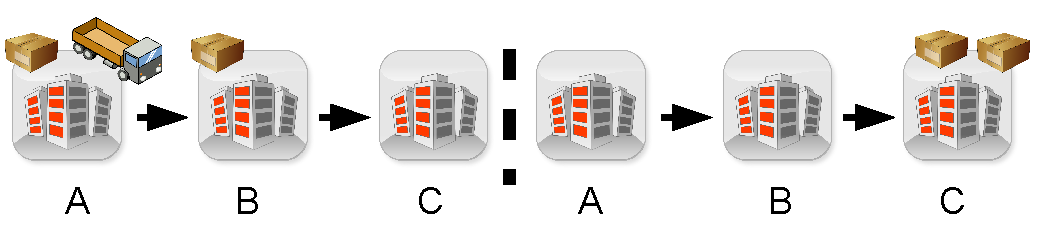
\includegraphics[scale=0.65]{figures/l10/plan-example.pdf}
\begin{itemize}
	\item Initial State
	\begin{itemize}
	\item There is a truck and a package in city A
	\item There is a package in city B
	\end{itemize}
	\item Goal
	\begin{itemize}
	\item There are two packages in city C
	\end{itemize}
	\item Possible Actions
	\begin{itemize}
	\item (Un)loading packages from/on the truck, driving between cities
	\end{itemize}
\end{itemize}
\end{frame}

\begin{frame}{Formalizing Planning}
\begin{block}{Planning Problem Definition -- SAS+ formalism}
A planning problem instance $\Pi$ is a tuple $(\mathcal{X}, \mathcal{A}, s_I, s_G)$ where
\begin{itemize}
	\item $\mathcal{X}$ is a set of multivalued variables with finite domains.
	\begin{itemize}
	\item each variable $x\in \mathcal{X}$ has a finite possible set of values $dom(x)$
	\end{itemize}
	\item $\mathcal{A}$ is a set actions. Each action $a\in\mathcal{A}$ is a tuple $(pre(a),eff(a))$
	\begin{itemize}
	\item $pre(a)$ is a set of preconditions of action $a$
	\item $eff(a)$ is a set of effects of action $a$
	\item both are sets of equalities of the form $x=v$ where $x\in\mathcal{X}$ and $v\in dom(x)$	
	\end{itemize}
	\item $s_I$ is the initial state, it is a \textbf{full} assignment of the variables in $\mathcal{X}$
	\item $s_G$ is the set of goal conditions, it is a set of equalities (same as $pre(a)$ and $eff(a)$)
\end{itemize}
\end{block}
\end{frame}

\begin{frame}{Formalizing Planning II}
\begin{block}{World State}
A state is full assignment of the variables in $\mathcal{X}$ (each variable $x \in \mathcal{X}$
has exactly one value assigned from its domain $dom(x)$. A state can be represented as a set of equalities.
\end{block}
The initial state $s_I$ is a state. A state $s$ is a goal state if $s_G \subseteq s$
\begin{block}{Applicable Actions}
An action $a\in\mathcal{A}$ is applicable in the state $s$ if $pre(a) \subseteq s$
\end{block}
\begin{block}{Applying an Action}
When an action $a\in\mathcal{A}$ is applied in the state $s$ it changes to the state $s'$
such that $eff(a)\subseteq s'$ and the difference between $s$ and $s'$ is minimal
(only variables used in $eff(a)$ are changed).
\end{block}
\end{frame}


\begin{frame}{Formalizing Planning III}
\begin{block}{A Plan}
A plan for $P$ for a planning problem $\Pi = (\mathcal{X}, \mathcal{A}, s_I, s_G)$ is sequence of
actions $a_1, a_2, \dots a_n$ such that
\begin{itemize}
	\item $\forall i$ $a_i \in \mathcal{A}$
	\item let $s_1 = s_I$ and $s_{i+1} = apply(s_i,a_i)$
	\item $a_i$ is applicable in $s_i$
	\item $s_G \subseteq s_{n+1}$
\end{itemize}
If $P=\{a_1, a_2, \dots a_n\}$ then $n$ is the lenght of the plan $P$.
\end{block}
An optimal plan is a plan of shortest length.
\end{frame}

\begin{frame}{Trucking Example}
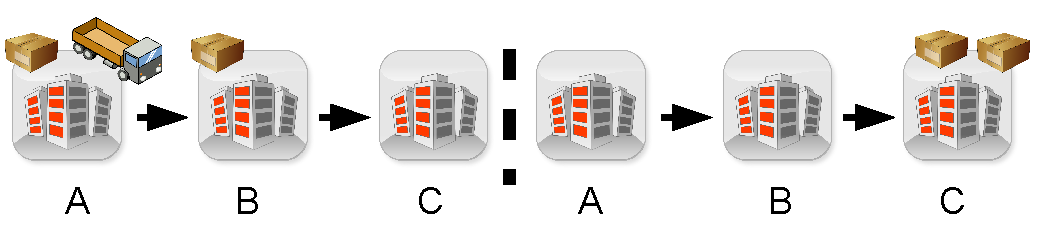
\includegraphics[scale=0.65]{figures/l10/plan-example.pdf}
\begin{itemize}
	\item variables: Truck Location $T$, $dom(T)=\{A,B,C\}$, Package Locations $P_1$ and $P_2$,
	$dom(P_1)=dom(P_2)=\{A,B,C,T\}$
	\item Initial state: $\{T=A, P_1=A, P_2=B\}$
	\item Goal: $\{P_1=C, P_2=C\}$
	\item Actions: $load(P_i,L) = (\{T=L, P_i=L\}, \{P_i=T\})$
	$unload(P_i,L) = (\{T=L, P_i=T\}, \{P_i=L\})$
	$drive(L_1,L_2) = (\{T=L_1\},\{T=L_2\})$ where $i\in\{1,2\}$ and $L,L_1,L_2\in \{A,B,C\}$
\end{itemize}
\end{frame}

\begin{frame}{Trucking Example}
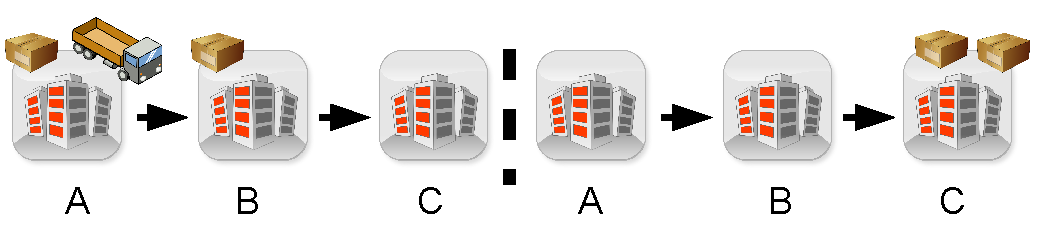
\includegraphics[scale=0.65]{figures/l10/plan-example.pdf}\\

\begin{columns}
\begin{column}{0.5\textwidth}
World State
\begin{itemize}
	\item $T=A, P_1=A, P_2=B$
	\item $T=A, P_1=T, P_2=B$
	\item $T=B, P_1=T, P_2=B$
	\item $T=B, P_1=T, P_2=T$
	\item $T=C, P_1=T, P_2=T$
	\item $T=C, P_1=C, P_2=C$
\end{itemize}
\end{column}
\begin{column}{0.5\textwidth}
The Plan
\begin{itemize}
	\item $load(P_1,A)$
	\item $drive(A,B)$
	\item $load(P_2,B)$
	\item $drive(B,C)$
	\item $unload(P_1,C)$, $unload(P_1,C)$
\end{itemize}
\hspace{1em}
\end{column}
\end{columns}
\end{frame}

\begin{frame}{Sokoban Example}
\begin{columns}
\begin{column}{0.5\textwidth}
\begin{itemize}
	\item Initial State
	\begin{itemize}
	\item There is a worker and a bunch of boxes
	\end{itemize}
	\item Goal
	\begin{itemize}
	\item All the boxes must be in goal positions
	\end{itemize}
	\item Possible Actions
	\begin{itemize}
	\item moving with the worker
	\item pushing a box
	\end{itemize}
	\item Forbidden
	\begin{itemize}
	\item to pull boxes
	\item move through walls or boxes
	\end{itemize}
\end{itemize}
\end{column}
\begin{column}{0.5\textwidth}
\url{http://wki.pe/Sokoban}

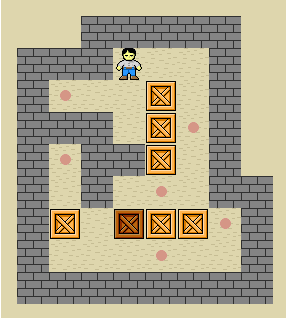
\includegraphics[scale=0.45]{figures/l10/sokoban.png}
\end{column}
\end{columns}
\end{frame}


\begin{frame}{Encoding Sokoban}
\begin{columns}[onlytextwidth,T]
\column{0.65\textwidth}
World State
\begin{itemize}
	\item Variables -- 
	For each location we have variable, the domain is WORKER, BOX, EMPTY
	\item Initial State -- assign values based on the picture
	\item Goal -- goal position variables have value BOX
\end{itemize}

Actions: move and push for each possible location
 
\begin{itemize}
	\item $push(L_1,L_2,L_3)=(\{L_1=W, L_2=B, L_3=E\},$\\
	 \hspace{9em}$\{L_1=E, L_2=W, L_3=B\})$
	\item $move(L_1,L_2)=(\{L_1=W, L_2=E\},\{L_1=E,L_2=W\})$
\end{itemize}
\column{0.35\textwidth}
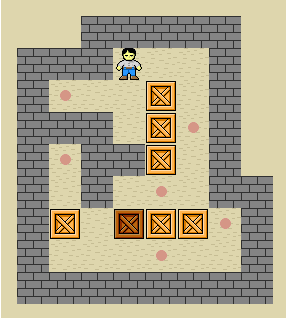
\includegraphics[scale=0.45]{figures/l10/sokoban.png}
\end{columns}
\end{frame}


\begin{frame}{Encoding Planning into CNF}
Is that even possible?
\end{frame}

\begin{frame}{Encoding Planning into CNF}
\begin{itemize}
	\item We cannot encode the existence of a plan in general
	\item But we can encode the existence of plan up to some length
\end{itemize}
\pause
\begin{block}{SATPLAN Algorithm}
\begin{itemize}
	\item INPUT: a planning problem $\Pi$
	\item OUTPUT: a plan $P$
\end{itemize}
\textbf{for} $m:=1,2,\dots$ \textbf{do}\\
\hspace{1em} $F = \operatorname{encodePlanExists}(\Pi,m)$\\
\hspace{1em} \textbf{if} solver.isSat($F$) \textbf{then}\\
\hspace{1em}\hspace{1em}\textbf{return} extractPlan($\Pi,m,$ solver.solution)\\
\end{block}
\end{frame}


\begin{frame}{Encoding Planning into CNF}
\begin{block}{The Task}
Given a planning problem instance $\Pi = (\mathcal{X}, \mathcal{A}, s_I, s_G)$ and $k\in \mathbb{N}$
construct a CNF formula $F$ such that $F$ is satisfiable if and only if there is plan of length $k$
for $\Pi$.
\end{block}
\pause
We will need two kinds of variables
\begin{itemize}
	\item Variables to encode the actions:\\
	$a_i^t$ for each $t \in \{1,\dots,k\}$ and $a_i \in \mathcal{A}$
	\item Variables to encode the states:\\
	$b_{x=v}^t$ for each $t \in \{1,\dots,k+1\}$, $x \in \mathcal{X}$ and $v \in dom(x)$
\end{itemize}
\vspace{1em}
In total we have $k|\mathcal{A}| + (k+1)\sum_{x \in \mathcal{X}} dom(x)$ variables
\end{frame}


\begin{frame}{Encoding Planning into CNF}
We will need 8 kinds of clauses
\begin{itemize}
	\item The first state is the initial state
	\item The goal conditions are satisfied in the end
	\item Each state variable has at least one value
	\item Each state variable has at most one value
	\item If an action is applied it must be applicable
	\item If an action is applied its effects are applied in the next step
	\item State variables cannot change without an action between steps
	\item At most one action is used in each step
\end{itemize}
\end{frame}



\begin{frame}{Encoding Planning into CNF}
The first state is the initial state
\begin{equation}
\begin{split}
&(b_{x=v}^1) \\
\forall (x&=v) \in s_I
\end{split}
\end{equation}

The goal conditions are satisfied in the end

\begin{equation}
\begin{split}
&(b_{x=v}^{n+1}) \\
\forall (x&=v) \in s_G
\end{split}
\end{equation}
\end{frame}

\begin{frame}{Encoding Planning into CNF}
Each state variable has at least one value
\begin{equation}
\label{eq2-1}
\begin{split}
&(b_{x=v_1}^t \vee b_{x=v_2}^t \vee \dots \vee b_{x=v_d}^t) \\
\forall x \in X,\; &\operatorname{dom}(x)=\{v_1, v_2, \dots, v_d\},\; \forall t \in \{1,\dots,k+1\}
\end{split}
\end{equation}

Each state variable has at most one value

\begin{equation}
\label{eq2-2}
\begin{split}
&(\neg b_{x=v_i}^t \vee \neg b_{x=v_j}^t)\\
\forall x \in X,\; v_i \neq v_j,\;& \{v_i,v_j\} \subseteq \operatorname{dom}(x),\; \forall t \in \{1,\dots,k+1\}
\end{split}
\end{equation}
\end{frame}


\begin{frame}{Encoding Planning into CNF}
If an action is applied it must be applicable
\begin{equation}
\label{eq2-3}
\begin{split}
&(\neg a^t \vee b_{x=v}^t)\\
\forall a \in \mathcal{A},\; \forall (x=&v)\in \operatorname{pre}(a),\; \forall t \in \{1,\dots,k\}
\end{split}
\end{equation}
If an action is applied its effects are applied in the next step
\begin{equation}
\label{eq2-4}
\begin{split}
&(\neg a^t \vee b_{x=v}^{t+1})\\
\forall a \in \mathcal{A},\; \forall (x=&v)\in \operatorname{eff}(a),\; \forall t \in \{1,\dots,k\}
\end{split}
\end{equation}
\end{frame}

\begin{frame}{Encoding Planning into CNF}

State variables cannot change without an action between steps

\begin{equation}
\label{eq2-5}
\begin{split}
&(\neg b_{x=v}^{t+1} \vee b_{x=v}^{t} \vee a_{s_1}^t \vee \dots \vee a_{s_j}^t)\\
\forall x \in X,\; \forall v \in \operatorname{dom}(x)&, \; 
\operatorname{support}(x=v)=\{a_{s_1},\dots,a_{s_j}\},\; \forall t \in \{1,\dots,k\}
\end{split}
\end{equation}
By $\operatorname{support}(x=v) \subseteq \mathcal{A}$ we mean the set of \emph{supporting actions}
of the assignment $x=v$, i.e., the set of actions that have $x=v$ as one of their effects.
\end{frame}


\begin{frame}{Encoding Planning into CNF}
At most one action is used in each step
\begin{equation}
\label{eq2-6}
\begin{split}
&(\neg a_{i}^t \vee \neg a_{j}^t)\\
\forall \{a_i,a_j\} \subseteq  \mathcal{A},\; &a_i \neq a_j \; \forall t \in \{1,\dots,k\}
\end{split}
\end{equation}
\end{frame}


\begin{frame}{Encoding Planning into CNF}
\begin{block}{The Task Solved}
Given a planning problem instance $\Pi = (\mathcal{X}, \mathcal{A}, s_I, s_G)$ and $k\in \mathbb{N}$
a CNF formula $F$, which is a conjunction of all the above described clauses is satisfiable if and only if there is plan of length $k$ for $\Pi$.
\end{block}
Optimizations
\begin{itemize}
\item Better encoding of at-most-one
\item Allowing several actions in each step
\item Encoding variable transitions instead of variable values
\end{itemize}
\end{frame}

\begin{frame}{SAT is NP-Hard -- proof sketch}
\begin{itemize}
	\item Let $M$ be a non-deterministic Turing machine that accepts an input $x$ in $P(|x|)$ time,
	where $P$ is a polynomial function.
	\begin{itemize}
	\item $M$ on $x$ will use at most $P(|x|)$ tape entries
	\end{itemize}
	\item $M$ on input $x$ as a SAS+ planning problem $\Pi$
	\begin{itemize}
	\item State variables are the state of the TM and the  $P(|x|)$ tape entries
	\item The transition function table is encoded as actions
	\item Initial state: tape contains input, TM state is initial state
	\item Goal state: TM state is an accepting state
	\end{itemize}
	\item Encode $\Pi$ for plan lenght $k=P(|x|)$ into a CNF formula $F_k$
	\item $F_k$ is SAT if and only if $M$ accepts $x$ in $P(|x|)$ time
	\item $F_k$ has polynomial size w.r.t. to $M$ and $x$
\end{itemize}
\end{frame}


\begin{frame}{Planning with incremental SAT}
\begin{itemize}
	\item we are solving a sequence of similar formulas
	\item how do they differ?
	\item how to use an incremental solver in this case?
\end{itemize}
\end{frame}

\begin{frame}{Planning with incremental SAT}
\begin{itemize}
\item The formula $F_k$ is the subset of $F_{k+1}$ except for the goal clauses.
\item The goal clauses will be added as removable (in this case, since they are unit, we can just assume
them)
\end{itemize}
\begin{block}{Incremental SATPLAN Algorithm}
\begin{itemize}
	\item INPUT: a planning problem $\Pi$
	\item OUTPUT: a plan $P$
\end{itemize}
$S = \operatorname{initSolver}()$ \\
$\operatorname{addInitialStateClauses}(S)$\\
\textbf{for} $m:=1,2,\dots$ \textbf{do}\\
\hspace{1em} $\operatorname{addClausesForStep}(m, S)$\\
\hspace{1em} $\operatorname{assumeGoalConditionsAtStep}(m, S)$\\
\hspace{1em} \textbf{if} satisfiable($S$) \textbf{then} \textbf{return} extractPlan($\Pi,m,$ getValues($S$))\\
\end{block}
\end{frame}

\begin{frame}{The DIMSPEC format}
\begin{itemize}
	\item Many other (than planning) problems have a similar structure
	\begin{itemize}
	\item for example bounded model checking
	\end{itemize}
	\item They can be specified using the DIMSPEC format
	\item DIMSPEC is four cnf formulas, where the \texttt{"p cnf <n> <m>"} line is replaced by:
	\begin{itemize}
	\item \texttt{i cnf <n> <m>} for the initial state specification ($n$ variables)
	\item \texttt{g cnf <n> <m>} for the goal state specification ($n$ variables)
	\item \texttt{u cnf <n> <m>} for the universal state specification ($n$ variables)
	\item \texttt{t cnf <n> <m>} for the specification of the transition (between two neigbhoring states) ($2n$~variables)
	\end{itemize}
\end{itemize}
\end{frame}

\begin{frame}{The DIMSPEC format example}
\texttt{c this is an example of a dimspec file}\\
\texttt{i cnf 5 3}\\
\texttt{-1 2 0}\\
\texttt{2 3 -5 0}\\
\texttt{4 0}\\
\texttt{g cnf 5 1}\\
\texttt{5 0}\\
\texttt{u cnf 5 2}\\
\texttt{-1 2 3 0}\\
\texttt{-3 4 5 0}\\
\texttt{t cnf 10 2}\\
\texttt{-2 7 8 0}\\
\texttt{-4 9 10 0}\\
\end{frame}

\begin{frame}{Planning as DIMSPEC}
\begin{itemize}
	\item Initial state specificaion clauses: $(b_{x=v})$ added $\forall (x=v) \in S_I$
	\item Goal state specificaion clauses: $(b_{x=v})$ added $\forall (x=v) \in S_G$
	\item Universal state specification clauses:
	\begin{itemize}
	\item $(b_{x=v_1} \vee b_{x=v_2} \vee \dots \vee b_{x=v_d})$ added
	$\forall x \in X$ where $\operatorname{dom}(x)=\{v_1, v_2, \dots, v_d\}$ -- at least one value
	\item $(\overline{b_{x=i}} \vee \overline{b_{x=j}})$ added
	$\forall x \in X\; i \neq j \in \operatorname{dom}(x)$ -- at most one value
	\item $(\overline{a} \vee b_{x=v})$ added $\forall a \in \mathcal{A},\; 
	\forall (x=v)\in \operatorname{pre}(a)$ -- action preconditions
	\item $(\overline{a_{i}} \vee \overline{a_{j}})$ added $\forall i \neq j$ -- at most one action
	\end{itemize}
	\item Transition specification clauses
	\begin{itemize}
	\item $(\overline{a} \vee b_{x=v}')$ added $\forall a \in \mathcal{A},\; 
	\forall (x=v)\in \operatorname{eff}(a)$ -- action effects
	\item $(\overline{b_{x=v}'} \vee b_{x=v} \vee a_{s_1} \vee \dots \vee a_{s_j})$ added
	$\forall x \in X,\; \forall v \in \operatorname{dom}(x)$ where
	$\operatorname{support}(x=v)=\{a_{s_1},\dots,a_{s_j}\}$ -- values cannot change without a reason
	\end{itemize}
\end{itemize}
\end{frame}

\begin{frame}{Solving DIMSPEC}
\begin{itemize}
\item Same as solving planning with incremental SAT
\end{itemize}
\begin{block}{The Basic DISMPEC Solving Algorithm}
\begin{itemize}
	\item INPUT: a DIMSPEC problem
	\item OUTPUT: a truth assignment
\end{itemize}
$S = \operatorname{initSolver}()$ \\
$\operatorname{addInitialStateClauses}(S)$\\
\textbf{for} $m:=1,2,\dots$ \textbf{do}\\
\hspace{1em} $\operatorname{addUniversalConditionsWithRenaming}(m, S)$\\
\hspace{1em} \textbf{if} $m > 1$ \textbf{then} $\operatorname{addTransitionalConditionsWithRenaming}(m, S)$\\
\hspace{1em} $\operatorname{assumeGoalConditionsWithRenaming}(m, S)$\\
\hspace{1em} \textbf{if} satisfiable($S$) \textbf{then} \textbf{return} getValues($S$)\\
\end{block}
\end{frame}

\end{document}
